\chapter{Resultados} \label{ch:Resultados}
	%  Os resultados seguem a metodologia

	% Definir qual o top_k utilizado
	% Verificar em Were2014 novamente
	% Padrão do zettair (se não me engano é 20)
	% Artigo de fulano não diz

	% Capítulo de Resultados 

	% -> Introdução: "Este capítulo apresenta os resultados obtidos e discute-os..." 
	Este capítula apresenta os resultados obtidos neste estudo investigativo do desempenho de atributos de RI em classificadores de Mineração de Texto.

	Nas subseções a seguir primeiro é abordada a configuração experimental utilizada para realizar o estudo, e logo em seguida é apresentada uma visão geral das soluções selecionadas dos corpus DB\_AUTHORPROF e DB\_HYPERPARTISAN, onde o pré-processamento realizado e os classificadores utilizados em cada uma das soluções são descritos brevemente.
	Por fim, são apresentados os resultados mensurados por meio das medidas escolhidas para avaliação de desempenho, na Seção \ref{sec:DesempenhoFerramentas} estão as medidas de desempenho das ferramentas de armazenamento e indexação, e na Seção \ref{sec:DesempenhoClassificadores} são expostas as medidas de desempenho dos classificadores.

	% Na subseção a seguir são abordados os resultados referentes às ferramentas de indexação.
	% Na subseção posterior são abordados os resultados referente aos desempenho das variáveis de RI em classificadores.

	\section{Configuração experimental} \label{sec:ConfiguraçãoExperimental}
	% 4.0 Setup experimental 

		Para programação e execução dos experimentos foi utilizado o sistema computacional disponível para o autor, com a configuração disposta na Tabela \ref{tab:sistema-computacional}.

		\begin{table}[ht]
    \centering
    \caption{Configuração do computador de mesa utilizado neste estudo.}
    \begin{adjustbox}{max width={\textwidth},keepaspectratio}%
    \begin{tabular}{|l|l|}
        \hline
        % \textbf{Posição}  
        % & \makecell[l]{\textbf{Equipe}}
        % & \makecell[l]{\textbf{Repositório de código no site \url{https://github.com/}}}
        % \\ \hline
        Processador
        & Intel(R) Core(TM) i7-4770 CPU @ 3.40GHz
        \\ \hline
        Memória RAM
        & 32370 MB
        \\ \hline
        Sistema Operacional
        & Linux Mint 19.2 Tina
        \\ \hline
        Placa-mãe
        & Gigabyte Z97-D3H
        \\ \hline
        Gráficos
        & Mesa DRI Intel(R) Haswell Desktop
        \\ \hline
        Disco
        & HP SSD EX920 512GB
        \\ \hline
    \end{tabular}
    \end{adjustbox}
    \legend{\ABNTEXfontereduzida \textbf{Fonte:} O autor.}
    \label{tab:sistema-computacional}
\end{table}
		
		As ferramentas de armazenamento e indexação receberam os mesmos parâmetros de refinamento na configuração de suas funções BM25, sendo estes configurados em $k_1 = 1.2$, $k_3 = 0$ e $b = 0.75$.
		O parâmetro $k_3$ (escalonar frequência de termos na consulta) é exclusivo do Zettair, as demais ferramentas não implementam este parâmetro.

		% Fixação do número aleatório do Python e das bibliotecas utilizadas nas soluções, quando isto não era feito originalmente, para permitir reprodutibilidade exata dos resultados obtidos.
		% [ ] FOOTNOTE DO VSCODIUM?
		O ambiente de programação utilizado foi o VSCodium e a linguagem de programação utilizada foi o Python 3.7.5.
		Para permitir reprodutibilidade dos resultados obtidos, o gerador de número aleatórios (RNG) do ambiente do Python, assim como os RNGs das bibliotecas utilizadas pelas soluções, tiveram as suas sementes de geração fixadas.

		Todo os códigos fontes dos scripts Python criados para este estudo estão disponíveis em um repositório de código online e púbilco criado pelo autor, acessível pelo seguinte link: \hyperlink{https://github.com/ruanmed/tcc-ii-ir-features-text-mining/}{https://github.com/ruanmed/tcc-ii-ir-features-text-mining/}.

	\section{Visão geral das soluções selecionadas e adaptações feitas} \label{sec:VisãoSoluçõesEAdaptações}
		% Falar brevemento sobre o pré-processamento;
		% Falar sobre o classificador utilizado; e
		% Indicar o Notebook de cada solução para mais detalhes
		As soluções selecionadas para reprodução e posterior adição dos atributos de RI utilizam de diferentes técnicas para pré-processamento dos corpus e também de classificadores diferentes, tornando necessário, em alguns casos, ajustes antes da adição dos atributos de RI.

		Nas subseções a seguir são brevemente abordadas as soluções 1\_bertha e 4\_tom do corpus DB\_HYPARTISAN, e a solução 2\_daneshvar18 do corpus DB\_AUTHORPROF.

		\subsection{Corpus DB\_HYPERPARTISAN}
			O corpus DB\_HYPERPARTISAN possui dois conjuntos de dados, o primeiro com 750 mil artigos classificados por enviesamento do editor, e o segundo com 645 artigos rotulados como hiperpartidários ou não com consenso entre avaliadores via \textit{crowdsourcing}.
			O objetivo da competição que utilizou esse corpus era classificar artigos como hiperpartidários ou não, e assim os participantes puderam utilizar os dois conjuntos para fazer suas avaliações. 
			No entanto, a utilização dos 750 mil artigos classificados por enviesamento de editor não foram úteis para ajudar na classificação, e das duas soluções selecionadas nenhuma delas utilizou esses 750 mil artigos nos seus modelos finais, pois utilizar a informação de editor em conjunto reduziu o desempenho de seus classificadores \cite[p.~840]{jiang-etal-2019-team} pois segundo \citeonline[p.~1067]{yeh-etal-2019-tom} o conjunto de dados classificado por enviesamento do editor possui muito ruído.

			O conjunto de validação final da competição não foi disponibilizado ao público, portanto para reprodução das soluções foi necessário dividir o conjunto de 645 artigos em treinamento e validação pelo método de \textit{holdout}, ficando assim com 430 artigos para treinamento e 215 artigos para teste. 
			Essa divisão foi feita de modo que as classes mantiveram-se com o mesmo balanceamento do conjunto original (37\% dos artigos hiperpartidário e 63\% não hiperpartidários).

			Então, os 430 artigos foram indexados em todas as ferramentas de indexação permitindo a geração dos atributos de RI posteriormente.
			A indexação foi feita com auxílio da classe \textit{IndexToolManager} criada pelo autor, que é abordada com detalhes na seção de desempenho das ferramentas de armazenamento e indexação.
			
			\subsubsection{Solução 1\_bertha}
				A solução da equipe Bertha von Suttner (4\_bertha) para essa tarefa da \textit{SemEval 2019} consiste em uma abordagem de classificação com uma Rede Neural Convolucional (\textit{Convolutional Neural Network}, CNN) e o pré-processamento dos documentos do corpus em uma representação destes por meio de uma Rede ESRC (\textit{ELMo Sentence Representation Convolutional Network}), uma representação sugerida e nomeada pela equipe.

				A representação na Rede ESRC é uma alternativa a representação usual dos documentos por termos (ou \textit{tokens}).
				Essa representação consiste no cálculo da média dos agregados ELMo para os documentos, a nível de frase, e cada documento é representado como uma sequência desses agregados, que são vetores de tamanho de 1024 \textit{floats}. 
				Na implementação da solução cada documento é limitado a ocupar até 200 vetores de tamanho 1024, sendo então cada documento padronizado com forma 200 x 1024.
				ELMo é uma representação de palavras com contextualização profunda, que modela características complexas de uso das palavras, como sintaxe e semântica, e o uso dessas palavras em contextos linguísticos \cite{ELMoDBLP:journals/corr/abs-1802-05365}.

				A CNN do classificador consiste de 5 camadas convolucionais paralelas internamente que recebem como entrada os agregados ELMo, essas 5 camadas convolucionais se conectam a camada de saída da rede neural, com função de ativação sigmoid, mais detalhes da implementação da CNN podem ser vistos em \citeonline{jiang-etal-2019-team}.

				Para adicionar os 6 atributos de RI à rede foi embutido ao final de cada representação de documento 6 vetores de tamanho 1024, preenchidos pelo valor calculado de cada atributo para o respectivo documento, resultando em documentos com forma 206 x 1024.
				A adaptação da solução está ilustrada na Figura XX.
				
				% \begin{figure}[ht]
    \centering
    \caption{Arquitetura de sistema da solução 1\underscore{}bertha após adaptação.}
    \begin{center}
        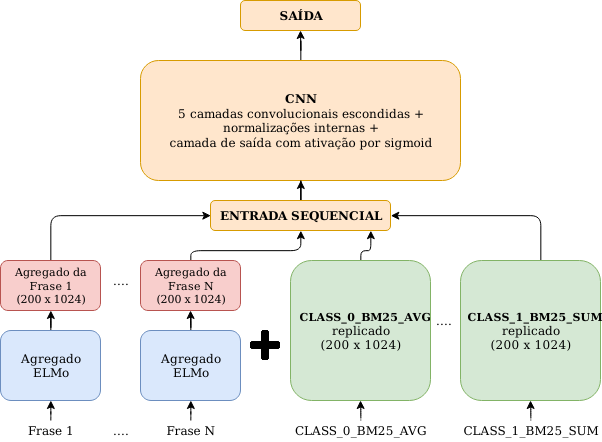
\includegraphics[width=0.75\textwidth]{img/1-bertha-arquitetura-com-ri.png}
    \end{center}
    \vspace{-0.5cm}
    \legend{\ABNTEXfontereduzida \textbf{Fonte:} O autor.}
    \label{fig:1-bertha-arquitetura-com-ri}
\end{figure}

				% \ref{fig:1-bertha-arquitetura-com-ri}
				A Figura XX é baseada na figura de representação de arquitetura do sistema apresentada no artigo de descrição da solução da equipe \cite{jiang-etal-2019-team}, alguns detalhes da CNN são abstraídos e os atributos de RI adicionados estão representados em verde.

			\subsubsection{Solução 4\_tom}
				A solução da equipe Tom Jumbo-Grumbo (4\_tom) utilizou de dois classificadores, um de Regressão Logística e outro de Máquinas de Vetor de Suporte (SVMs), sendo o utilizado no modelo final o classificador SVC (C-Support Vector Classification) da biblioteca sklearn para Python.
				Uma SVM funciona transformando os dados de treinamento para uma dimensão maior e então executa uma busca pelo melhor limite de decisão, chamado de hiperplano, para separar as classes \cite[p.~408]{Han:2011:DMC:1972541}.
				Em especial, o classificador SVC da biblioteca sklearn possui um parâmetro de regularização de sua função de custo (parâmetro chamado de C) que deve ser estritamente positivo, o valor padrão é definido como $C = 1.0$, no entanto a solução da equipe, conforme disposto no código fonte disponível online, utilizou $C = 0.9$ após uma análise com diferentes valores.

				No pré-processamento, a equipe utilizou três estratégias para converter os documentos em atributos para o classificador.
				A primeira foi de criar vetores baseados na frequência dos termos, descartando termos que apareçam em mais de 90\% dos documentos e utilizando os 50 mil termos mais frequentes dos que sobrarem, guardando o valor tf-idf para cada termo respectivo ao documento.
				A segunda foi treinar um modelo PV-DM para gerar os atributos referentes a cada documento.
				E a terceira utilizou um agregado pré-treinado em textos da Wikipédia com o algoritmo GloVe, que, similarmente aos agregados ELMo, tentam também inferir o significado das palavras dos documentos.

				A arquitetura com melhor resultado foi a utilização dos atributos GloVe com o classificador SVM da biblioteca sklearn.
				Os documentos são convertidos para os vetores GloVe pré-treinados a partir se suas primeiras 1000 palavras, esses vetores GloVe possuem 300 dimensões por palavra, o que resultaria numa representação com forma de 1000 x 300, no entanto o vetor final que representa cada documentos é a média dos vetores de palavras respectivos.

				Para adicionar os 6 atributos de RI foram embutidos, ao final de cada representação de documento, estes foram calculados para os respectivos documentos e embutidos no vetor GloVe do documento, resultando em documentos representados por 306 dimensões, ou 306 atributos.
				A arquitetura da solução adaptada está ilustrada na Figura XX.
				% \ref{fig:4-tom-arquitetura-com-ri}
				% \begin{figure}[h]
    \centering
    \caption{Arquitetura de sistema da solução 4\_tom após adaptação.}
    \begin{center}
        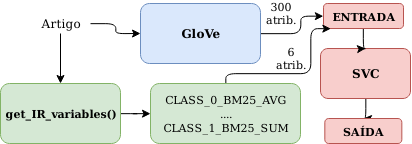
\includegraphics[width=0.68\textwidth]{img/4-tom-arquitetura-com-ri.png}
    \end{center}
    \vspace{-0.5cm}
    \legend{\ABNTEXfontereduzida \textbf{Fonte:} O autor.}
    \label{fig:4-tom-arquitetura-com-ri}
\end{figure}

		\subsection{Corpus DB\_AUTHORPROF}
			O corpus DB\_AUTHORPROF consiste de \textit{tweets} de autores em três línguas diferentes, inglês, espanhol e árabe.
			Para avaliação dos atributos de RI o escopo de melhoria de desempenho foram considerados somente os classificadores das soluções para os autores de língua inglesa, e as imagens não foram consideradas.

			O conjunto de treinamento de autores da língua inglesa consiste de 300 mil \textit{tweets} de 3000 autores diferentes, e como o conjunto de validação final está disponível ao público, necessário somente solicitar o acesso, não foi necessário fazer o \textit{holdout} do conjunto de treinamento.
			O conjunto de validação da língua inglesa consiste de 190 mil tweets de 1900 autores.

			Os 300 mil \textit{tweets} foram indexados em todas as ferramentas de indexação permitindo a geração dos atributos de RI posteriormente para cada \textit{tweet} específico.

			\subsubsection{Solução 2\_daneshvar18}
			% baseou o seu pré-processamento em soluções das melhores equipes dos anos anteriores em tarefas da PAN CLEF
			%  O QUE É N-GRAM
				A solução de \citeonline{daneshvar:2018} utilizou um classificador SVM com diferentes tipos de $n$-grams de palavras e caracteres como atributos, e o melhor resultado obtido foi com a criação dos $n$-grams, posterior redução de dimensionalidade e então utilização do classificador LinearSVC da biblioteca sklearn para Python para criar o modelo de classificação.

				A adaptação da solução para adicionar os atributos de RI poderia ser feita adicionando os atributos antes ou depois da redução de dimensionalidade utilizada pela equipe.
				Os documentos inicialmente são representados por vetores de 1243271 dimensões, após a diminuição da dimensionalidade cada documento é representado por um vetor de 300 dimensões.
				No entanto, uma peculiaridade da solução está em como é feita a classificação, os 100 \textit{tweets} de cada autor são tratados como um único documento, pois o objetivo é classificar o gênero dos autores em homens ou mulheres.
				Como os \textit{tweets} foram indexados individualmente, então para adicionar os atributos de RI para cada autor foi feita a geração dos 6 atributos para todos os tweets e então estes foram agregados por autor.

				% \begin{figure}[ht]
    \centering
    \caption{Arquitetura de sistema da solução 2\underscore{}daneshvar18 após adaptação.}
    \begin{center}
        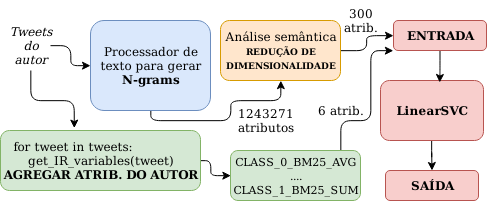
\includegraphics[width=0.75\textwidth]{img/2-daneshvar18-arquitetura-com-ri.png}
    \end{center}
    \vspace{-0.5cm}
    \legend{\ABNTEXfontereduzida \textbf{Fonte:} O autor.}
    \label{fig:2-daneshvar18-arquitetura-com-ri}
\end{figure}

				Por fim, os 6 atributos de RI agregados por autor foram embutidos ao final da representação dos documentos, resultando em documentos representados por 1243277 dimensões, e posteriormente também foi configurado outro experimento para embutir os atributos de RI somente após a redução de dimensionalidade, resultado em documentos represetados por 306 atributos.


		\subsection{Resumo das soluções} \label{sec:ResumoDasSoluções}
			Na Tabela \ref{tab:resumo-soluções} a seguir estão resumidas as principais características das soluções selecionadas.

			\begin{table}[!thb]
	%\huge
    \centering
    \caption{Resumo dos detalhes das soluções selecionadas.}
    \begin{adjustbox}{max width={\textwidth},keepaspectratio}%
    \begin{tabular}{|l|c|c|c|c|c|}
        % \toprule
        \hline
        \textbf{Solução}
        & \textbf{Pré-processamento} & \textbf{Núm. atrib.} & \textbf{Redução dim.} 
        & \textbf{Núm. atrib. após}  & \textbf{Classificador}
        \\ \hline
        1\underscore{}bertha        
        & ELMo          & 200 x 1024        & Não
        & 200 x 1024    & CNN (5 cam. esc.) 
        \\ \hline
        4\underscore{}tom
        & GloVe         & 300               & Não
        & 300           & SVC                
        \\ \hline
        2\underscore{}daneshvar18
        & N-gram palavras+caracteres & 1243271           & Sim
        & 300           & LinearSVC          
        \\ 
        \hline
        % \bottomrule
    \end{tabular}
    \end{adjustbox}
    \legend{\ABNTEXfontereduzida \textbf{Fonte:} O autor.}
    \label{tab:resumo-soluções} 
    % \legend{\textbf{Fonte:} O autor.}
\end{table}


	\section{Desempenho das ferramentas de armazenamento e indexação} \label{sec:DesempenhoFerramentas}
		Para cálculo das variáveis TIME\_INDEX e TIME\_QUERY, conforme sugeridas no Capítulo \ref{ch:MateriaisMétodos}, foi utilizada a linguagem de programação Python na qual foi implementada uma classe chamada \textit{IndexToolManager}, que abstrai a indexação e o cálculo das variáveis de RI com as ferramentas. 

		Esta classe foi central para todo o estudo.
		% Adicionar funcṍes importantes e cirtar código aqui?
		\subsection{Tempo de indexação}
			Para cálculo das medidas TIME\_INDEX foi criado um script python nomeado \texttt{time\_index.py}, o qual utilizou da classe \textit{IndexToolManager} em duas funções feitas para executar a indexação dos banco de dados, DB\_AUTHORPROF e DB\_HYPERPARTISAN, nas 3 ferramentas, ArangoDB, Elasticsearch e Zettair.
			As função principal do script \texttt{time\_index.py} é nomeada \textit{measure\_TIME\_INDEX}, este trecho do código pode ser vista a seguir.

			\sourcecodenolinenos{Função \textit{measure\_TIME\_INDEX} do script \texttt{time\_index.py}.}{function-measure-time-index}{python}{function-measure-TIME-INDEX.py}
			% \sourcecodeinline{python}{codes/function-measure-TIME-INDEX.py}

			Esta função é responsável por efetuar uma chamada à função \textit{index} com os parâmetros de tipo de indexação, corpus a ser indexado, e qual a ferramenta utilizada nesta indexação, além de uma identificação do experimento.
			A função \textit{index} faz os devidos tratamentos para chamar os métodos da classe \textit{IndexToolManager} responsáveis por fazer a indexação dos documentos do corpus especificado utilizando a ferramenta especificada, isso enquanto mensura o tempo que cada indexação levou e registra todas as operações num arquivo de texto.

			% Colocar o código fonte da função index aqui?
			
			Como as ferramentas ArangoDB e Elasticsearch se assemelham bastante a sistemas gerenciadores de bancos de dados completos, preparados, inclusive, para distribuição geográfica dos dados, há de ser citada essa grande diferença deles para o Zettair, este último que é somente um sistema para indexação em lotes e consulta local dos dados, não permitindo, por exemplo, adição de novos documentos em um índice. 
			A ação de inserção unitária é um procedimento comum em SGBDs. 			

			A operação de indexação foi executada de dois modos, em lote e unitária, sendo que o Zettair só permite a inserção em lote. 
			Na Figura \ref{fig:time-index-bulk} pode ser visto o tempo mensurado, em milissegundos gastos por documento, para inserção em lote dos documentos dos corpus em cada ferramenta.

			\begin{figure}[h]
    \centering
    \caption{Medidas de desempenho TIME\_INDEX mensuradas para as ferramentas de armazenamento e indexação, com inserções feitas em lote.}
    \begin{center}
        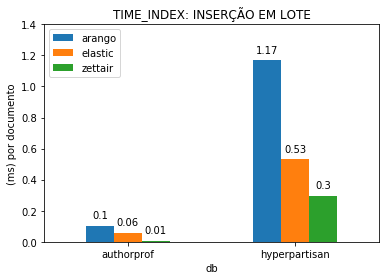
\includegraphics[width=0.75\textwidth]{img/time-index-bulk.png}
    \end{center}
    \vspace{-0.5cm}
    \legend{\ABNTEXfontereduzida \textbf{Fonte:} O autor.}
    \label{fig:time-index-bulk}
\end{figure}

			O Zettair é a ferramenta mais rápida para completar a indexação de ambos os corpus selecionados, levando somente 2,29 segundos para indexar os 300 mil documentos do corpus DB\_AUTHORPROF, menos de 0,01 milissegundos por documento.
			Dentre os SGBDs avaliados, o Elasticsearch supera o ArangoDB para inserções em lote, gastando 17,61 segundos para indexar os 300 mil \textit{tweets}, cerca de 0,06 milissegundos por documento.
			Nota-se ainda que a indexação do corpus DB\_HYPERPARTISAN é mais lenta quando se considera o tempo por documento inserido, porque, apesar do corpus DB\_AUTHORPROF ter um número bem maior de documentos, 300 mil em comparação com 645, cada artigo do DB\_HYPERPARTISAN é bem mais extenso que qualquer dos \textit{tweets} do DB\_AUTHORPROF.
			A mesma relação de velocidade entre as ferramentas observada para as inserções feitas com os documentos do DB\_AUTHORPROF se mantem para as inserções feitas com os documentos do DB\_HYPERPARTISAN, o Zettair é o mais rápido, e, dentre os SGBDs, o Elasticsearch é mais rápido que o ArangoDB.
			
			Para operação de inserção unitária, avaliada somente com o ArangoDB e Elasticsearch, foi levado em conta o tempo total para indexação de todos os documentos de cada corpus, inseridos em sequência, e posteriormente esses valores mensurados foram divididos pelo número de documentos.
			Na Figura \ref{fig:time-index-individual} estão dispostos os tempos totais para indexação de todos os documentos dos corpus com ambas ferramentas. 

			\begin{figure}[h]
    \centering
    \caption{Medidas de desempenho TIME\_INDEX mensuradas para as ferramentas de armazenamento e indexação, com inserções unitárias.}
    \begin{center}
        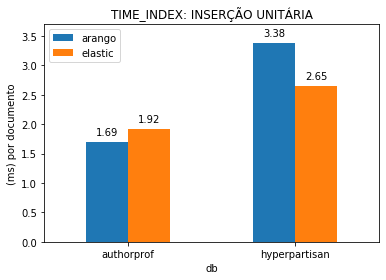
\includegraphics[width=0.75\textwidth]{img/time-index-individual.png}
    \end{center}
    \vspace{-0.5cm}
    \legend{\ABNTEXfontereduzida \textbf{Fonte:} O autor.}
    \label{fig:time-index-individual}
\end{figure}

			O ArangoDB teve um melhor desempenho para as inserções dos documentos do DB\_AUTHORPROF, com 1,69 milissegundos por documento, em contraste aos 1,92 milissegundos por documento do Elasticsearch.
			Porém, o Elasticsearch foi mais rápido para inserção dos documentos do DB\_HYPERPARTISAN, com 2,65 milissegundos por documento contra 3,38 milissegundos por documento do ArangoDB.		

			Percebe-se então que o ArangoDB se saiu um pouco melhor que o Elasticsearch na inserção de grande quantidade de documentos pequenos em sequência, evidênciado pelos tempos de inserção unitária da Figura \ref{fig:time-index-individual}.
			E pode-se supor que isto é derivado de alguma sobrecarga na operação de inserção unitária do Elasticsearch, ou talvez no custo de recálculo do índice que varia com o tamanho dos documentos inseridos, porém com um custo inicial maior, já que para inserção unitária dos documentos do DB\_HYPERPARTISAN, que são artigos extensos, o Elasticsearch teve melhor desempenho.
				
			No geral, o desempenho da indexação por inserção unitária fica abaixo da por inserção em lotes, como era esperado.

		\subsection{Tempo de consulta}
			Para medir o TIME\_QUERY utilizando cada ferramenta durante a execução das soluções foi necessário adaptar os códigos das soluções para fazer o registro do tempo que cada consulta, e posterior geração dos atributos de RI, levou.

			A fim de facilitar a geração dos atributos, foram implementados métodos na classe \textit{IndexToolManager} para que dado um texto seja cálculo direto das variáveis de RI já com as ferramentas específicas, como por exemplo o método \textit{arango\_get\_IR\_variables}.
			A utilização desses métodos pode ser visto no trecho disposto a seguir do script Python \texttt{feat\_GloVe.ipynb} da solução 4\_tom adaptada.

			\sourcecodenolinenos{Trecho da adaptação feita ao script \texttt{feat\_GloVe.ipynb} da solução 4\_tom.}{time-query-calculation-4-tom}{python}{time-query-calculation-4-tom.py}

			Neste trecho, Código \ref{cmd:time-query-calculation-4-tom}, \textit{toolTest} é uma instância da classe \textit{IndexToolManager}, e assim esta classe que é responsável pelo cálculo das variáveis de RI, e o tempo de consulta leva em conta esse cálculo, como fica exposto pela posição das variáveis \textit{initial} e \textit{final}.

			O mesmo tipo de adaptação feito para a solução 4\_tom foi feito para as demais, e as medidas coletadas estão dispostas na Figura \ref{fig:time-query}.

			\begin{figure}[h]
    \centering
    \caption{Medidas de desempenho TIME\_QUERY mensuradas para consulta e criação dos 6 atributos de RI sugeridos, utilizando as ferramentas de armazenamento e indexação.}
    \vspace{-0.5cm}
    \begin{center}
        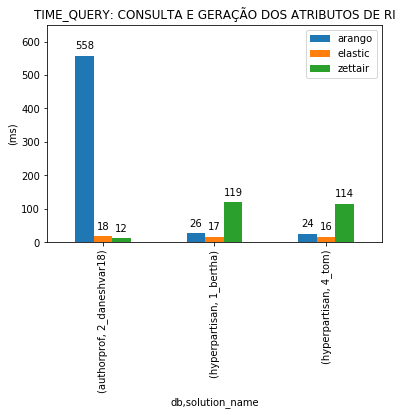
\includegraphics[scale=0.75]{img/time-query.png}
    \end{center}
    \vspace{-0.5cm}
    \legend{\ABNTEXfontereduzida \textbf{Fonte:} O autor.}
    \label{fig:time-query}
\end{figure}



	\section{Desempenho dos classificadores com atributos de RI} \label{sec:DesempenhoClassificadores}

		\subsection{DB\_HYPERPARTISAN}

			\begin{figure}[h]
    \centering
    \caption{Desempenho CLF\_ACC das soluções do corpus DB\_HYPERPARTISAN.}
    \vspace{-0.5cm}
    \begin{center}
        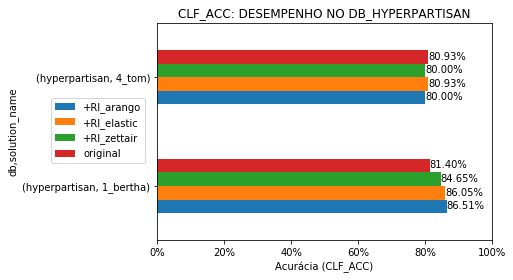
\includegraphics[scale=0.75]{img/clf-acc-bars-hyperpartisan.png}
    \end{center}
    \vspace{-0.5cm}
    \legend{\ABNTEXfontereduzida \textbf{Fonte:} O autor.}
    \label{fig:clf-acc-bars-hyperpartisan}
\end{figure}
			
			\begin{figure}[h]
    \centering
    \caption{Desempenho CLF\_F1 das soluções do corpus DB\_HYPERPARTISAN.}
    \vspace{-0.5cm}
    \begin{center}
        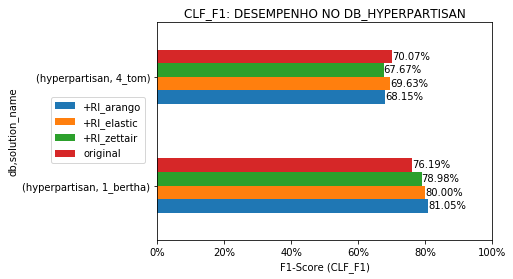
\includegraphics[scale=0.75]{img/clf-f1-bars-hyperpartisan.png}
    \end{center}
    \vspace{-0.5cm}
    \legend{\ABNTEXfontereduzida \textbf{Fonte:} O autor.}
    \label{fig:clf-f1-bars-hyperpartisan}
\end{figure}
		
		\subsection{DB\_AUTHORPROF}

	% Fluxograma das alterações feitas nos códigos com exemplos de trechos alterados
	% Rosalvo disse que é para colocar no Apêndice

	% Zettair, colocar detalhe dos modos de operação para consulta, iterativa e consulta única

	% ganho de informação das 6 variáveis nas soluções

	% Citar as técnicas só de um, descrições, citar algum livro ou página

	% Criar rede neural para comparar à solução do DB_AUTHORPROF à parte 

